\subsection{Stock Predictions}
Predicting stock prices based on historical data can be formulated as a time series forecast, consisting of sequential data and predicting the value of the next time step. Some of the many relevant data used for stock price predictions are everyday closing prices, price percentage changes, trading volume, fundamental business data like revenue and earnings or social sentiment. 
The stock market consists of many complex mechanisms that can be described by chaos theory as a nonlinear deterministic dynamical system \cite{KLIOUTCHNIKOV2017368, lawrence1997using}.

\subsection{Deep Neural Networks}
Deep neural networks have the ability to learn and model nonlinear, chaotic systems, therefore having great potential for solving financial prediction problems \cite{heaton2018deep}.



\subsection{Recurrent Neural Networks}
Recurrent Neural Networks (RNNs) are a specific type of deep neural networks, designed to handle and model sequential data, by memorizing past inputs.

\begin{figure}[h]
\centering
  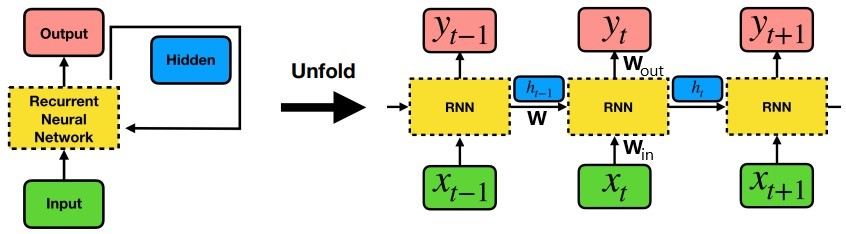
\includegraphics[width=1.0\columnwidth]{gfx/rnn}
  \hfill
 \caption{\cite{chen2020quantum} Each timestep, the next input value $x_t$ is put into the RNN, it returns the outputs $y_t$ and $h_t$, $h_t$ gets fed as a new input in the next round t+1.
 The output of a RNN block can be described as 
 \[h_t = f(x_t \cdot W_{in} + h_{t-1} \cdot W)\] 
 \[y_t = h_t + W_{out}\] 
 where $f$ is the activation function, and $W_{in}$, $W_{out}$, $W$ are the weights, that need to be optimized.}
 \label{fig:rnn}
\end{figure}

RNNs possess a multi-layer architecture, where each layer comprises a recurrent block. The key lies in the feedback mechanism of hidden states, where the information from all previous time steps is retained, predictions at any given moment depend on both the current input data and the information about the history of all past elements in the sequence. This architecture allows RNNs to capture and utilize information about the temporal evolution of the data. These attributes make them well-suited for applications involving sequential dependencies, like a time series of stock data, where a sequence of past days is used to predict the next day.
However, fundamental RNNs face a major problem: the weights are the same throughout the unfolding, which creates a problem called the vanishing gradient problem. 

\begin{figure}[h]
\centering
  \subfloat[Original.\label{subfig:original}]{%
  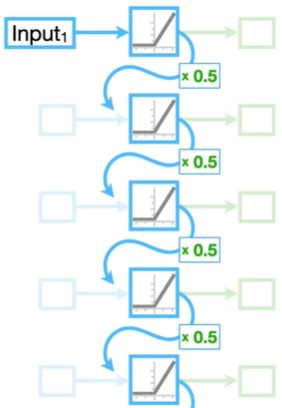
\includegraphics[width=.355\columnwidth]{gfx/vanishing_gradient}}
  \hfill
  \subfloat[Extended.\label{subfig:extended}]{%
  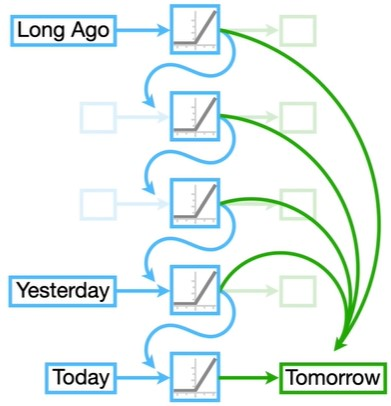
\includegraphics[width=.49\columnwidth]{gfx/extended_rnn}}
  \caption{\cite{starmer2022} With each iteration, the past inputs get multiplied with $W$. Unfolding many times creates small numbers close to 0, causing the gradient to vanish, which makes it hard to optimize the parameters (a). This can be countered by extending the model with a second separate memory component (b).}
  \label{fig:extending_rnn}
\end{figure}

\subsection{Long Short-Term Memory}
This problem can be avoided by upgrading to a LSTM neural network, that can capture long-term dependencies in sequential data. 
An LSTM cell has 3 inputs, the third being $c_{t-1}$, adding another memory path to the model. One functions as a short-term memory ($h_t$), the other as a long-term memory ($c_t$). This dual-memory structure erases the vanishing gradient problem and enhances numerical stability during training, resulting in more accurate predictions \cite{chen2020quantum}.

\begin{figure}[h]
\centering
  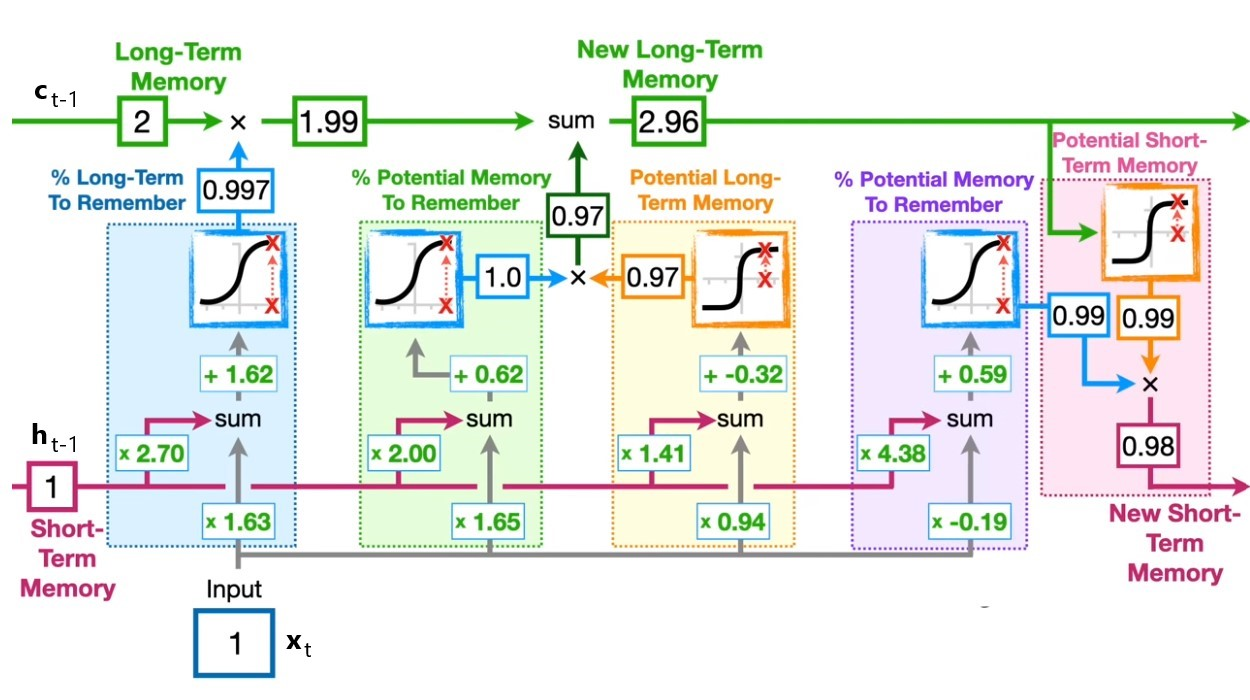
\includegraphics[width=1.0\columnwidth]{gfx/lstm_detailed}
  \hfill
 \caption{
 \cite{starmer2022} The blue block is called the forget gate and determines what percentage of the long-term memory remains. The green and yellow blocks form the input gate and decide, what is contributed to the long-term memory. The last two blocks form the output gate and compute a new short-term memory.
 }
 \label{fig:lstm}
\end{figure}


\subsection{Quantum Computing}
Quantum computing is an an emerging field of computer science that leverages the principles of quantum mechanics to enhance information processing. In contrast to traditional computers that represent data as binary digits or bits, quantum computers utilize quantum bits, or qubits \cite{yanofsky2008quantum}. These qubits are unique in that they can exist in multiple states simultaneously, a phenomenon known as superposition.

This capability of qubits allows quantum computers to process a vast amount of information more efficiently than classical computers. For instance, while a classical computer with $n$ bits can store and process one out of $2^n$  possible combinations at a time, a quantum computer with the same number of qubits can represent and process all $2^n$ combinations concurrently \cite{homeister2018quantum}.

The state of a qubit can be expressed as a linear combination of its base states $|$0⟩ and $|$1⟩, represented mathematically as
\begin{equation}
|\psi\rangle = \alpha|0\rangle + \beta|1\rangle,
\label{qubit}
\end{equation}
where $\alpha$ and $\beta$ are complex coefficients that satisfy the equation
\begin{equation}
|\alpha|^2 + |\beta|^2 = 1.
\end{equation}
When a qubit in the state of $\alpha \vert 0 \rangle + \beta \vert 1 \rangle$ is measured, its superposition collapses into one of its possible states, either $|$0⟩ or $|$1⟩, with probabilities determined by the coefficients $|\alpha|^2$ and $|\beta|^2$ respectively \cite{mcmahon2007quantum}. The quantum system transitions from a superposition of states to an actual classical state where the observable's value is precisely known \cite{nielsen2010quantum}.

\subsection{Variational Quantum Circuits}
Variational Quantum Circuits (VQCs) build on the principles of quantum circuits, essential in quantum computing. Like classical circuits, quantum circuits comprise quantum wires and gates. Each quantum wire carries a quantum bit (qubit), analogous to classical bits in classical circuits. Quantum gates perform unitary transformations on these qubits, mirroring the operations of classical gates on classical bits \cite{homeister2018quantum}.

A VQC, also known as a parametrized quantum circuit, is a unique quantum algorithm that integrates a classical optimization process to encode solutions to specific problems in a quantum state. The process in VQC involves several key steps: initially, classical data is inputted and converted into quantum states via quantum gates. This is followed by the entanglement of qubits using controlled gates and their rotation through parameterized rotation gates. These operations, forming a layer, can be repeated multiple times with varying parameters \cite{9144562}.

After processing, the qubits are measured, and the outcomes are decoded into classical information. The circuit parameters are then refined through classical optimization techniques like gradient descent, aiming to optimize the algorithm's objective function. These adjustments are made iteratively \cite{pennylane_variational_circuit_2022}.

\begin{figure}[!htbp]
\begin{center}
\begin{quantikz}
\lstick{\ket{0}} & \gate[wires=4][1.5cm]{U(x)} & \qw & \gate[wires=4][1.5cm]{V(\theta)} & \qw & \meter{} \\
\lstick{\ket{0}} && \qw && \qw & \meter{} \\
\lstick{\ket{0}} && \qw && \qw & \meter{} \\
\lstick{\ket{0}} && \qw && \qw & \meter{}
\end{quantikz}
\end{center}
\captionsetup{labelfont=bf, format=plain}
\caption{Variational Quantum Circuit. The general VQC structure contains three main parts: the $U(x)$-block is the state preparation part, the $V(\theta)$-block is the variational part containing trainable parameters $\theta$, and the quantum measurement layer.}
\label{fig:vqc}
\end{figure}

A notable feature of VQCs is their resilience to quantum noise \cite{Chen_2022}, making them particularly suitable for Noisy Intermediate-Scale Quantum era computers \cite{Preskill_2018}. Additionally, VQCs have shown promising results in various machine learning applications, including classification \cite{Chen_2021} and natural language processing tasks \cite{https://doi.org/10.48550/arxiv.2110.06510}.

